\chapter{B-trees}
\label{chapter:btree}
The B-tree is a very common data structure for storing sorted dictionaries.
B-trees are particularly useful where the external memory model is accurate,
because all information in every transferred block is actively used
in searching. For example, the ext4, Btrfs and NTFS filesystems use B-trees
to store directory contents and the MongoDB and MariaDB databases use B-trees
as indexes. Red-black trees, which are (in the left-leaning variant
described by \cite{left-leaning}) isomorphic to B-trees for $b=4$, are
commonly used to maintain in-memory dictionaries, for example in the GNU ISO
C++ Library as the implementation of the \texttt{std::map} STL template.
B-trees are also an optimal sorted dictionary data structure
for the external memory model assuming the only operation allowed on
keys is comparison.

B-trees are a generalization of balanced binary search trees.
Nodes of a B-tree keep up to $b$ key-value pairs in sorted order.
An inner node of a binary search tree with key $X$ contains two pointers
pointing to children with keys $< X$ and $\geq X$. In B-trees,
inner nodes contain $k\in[b/2;b)$ keys $K_1\ldots K_k$. There are $k+1$
child pointers in internal nodes: one for every interval
$[K_1;K_2),\ldots [K_{k-1};K_k)$, plus one for $(-\infty;K_1)$ and
$(K_k;\infty)$ each.
Leaf nodes of a B-tree store $[b/2;b)$ key-value pairs.
% TODO: check boundaries

\begin{figure}
\centering
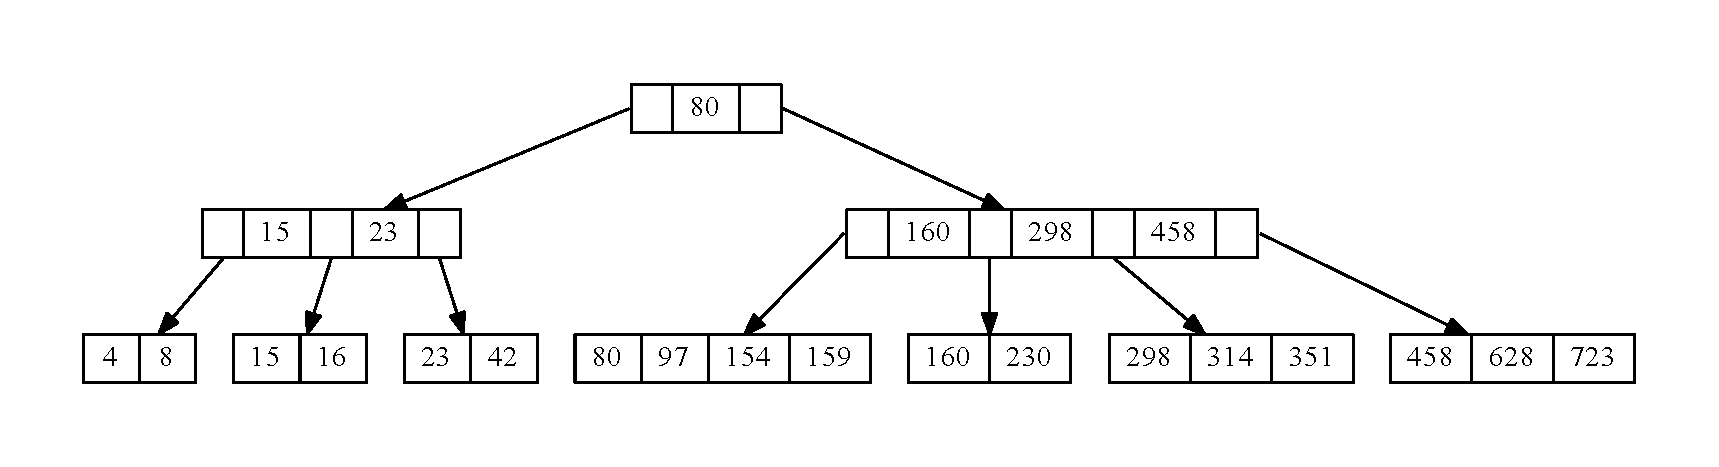
\includegraphics[width=\linewidth]{img/btree}
\caption{An example B-tree ($b=5$).}
\end{figure}

In binary search trees, searching for a key $K$ is performed by binary search.
Starting in the root node, we compare $K$ with the key stored in the node
and we go left or right depending on the result. If the current node's key
equals $K$, we fetch the value from the node and abort the search.

The process of finding a key-value pair in a B-tree generalizes this
by picking the child pointer corresponding to the only range that contains
the sought key $K$. To pick the child pointer, we can either do a simple
linear scan in $\Theta(b)$, or we can use binary search to get
$\Theta(\log b)$ if $b$ is not negligible.
Once we reach a leaf, we scan its keys and return the value for $K$
(if such a value exists).

To \textsc{Insert} a key-value pair in a B-tree, we first find the right
place to put the new key-value pair, and then walk back up the tree.
If an overfull node (with $\geq b$ keys) is encountered, it is split
to two nodes of $\leq b/2$ keys and a pointer to the new node is inserted into
the parent. When we split the root node, we immediately create a new
root node above the two resulting nodes.

Deletions employ a similar procedure: if the current node is underfull
(i.e. if it has $< b/2$ keys), it is merged with one of its siblings.
If there are not enough keys among the siblings for two nodes,
one of the siblings takes ownership of all keys and the other sibling
is recursively deleted from the parent.
The only exception is the root node, which may have $[1;b)$ keys.
If deleting from the root would leave the root with only one child
(and zero keys), we instead make the only child of the root the new root.

Thus, updates to the B-tree keep the number of keys of all nodes within
$[b/2;b$, so the depth of the tree is kept between $\log_b N$ and
$\log_{b/2} N$ and the \textsc{Find} operation takes time
$\Theta(\log b \cdot \log_b N)=\Theta(\log N)$. \textsc{FindNext} and
\textsc{FindPrevious} also take time $\Theta(\log N)$, but if they are invoked
after a previous \textsc{Find}, we can keep a pointer to the leaf containing
the key and accordingly adjust it to find the next or previous key, which runs
in $\O(1)$ amortized time. Thus, B-trees also allow scanning a contigous
range of keys of size $k$ in $\Theta(\log_b N + k)$ time.

The \textsc{Insert} and \textsc{Delete} operations may spend up to
$\Theta(b)$ time splitting or merging nodes on each level, so they run in
time $\Theta(b \cdot \log_b N)$.

The main benefit of B-trees over binary trees is the tunable parameter
$b$, which we can choose to be $\Theta(B)$. Practically, if the B-tree
is stored in a disk, $b$ can be tuned to fit one B-tree node in exactly one
physical block. Thus, in the external memory model, \textsc{Find},
\textsc{Insert} and \textsc{Delete} all take $\O(1)$ block transfers
on every level, yielding $\Theta(\log_B N)$ block transfers per operation.

This is optimal assuming the only allowed operation
on keys is comparison: reading a block of $\Theta(B)$ keys will only
give us $\log B$ bits of information, since the only useful operation
can be comparing the sought key $K$ with every key we retrieved.
We need $\log N$ bits to represent the index of the key-value pair we found,
so we need at least $\frac{\log N}{\log B}=\log_B N$ block transfers.
